% Provenance (never printed): cycle 2 "Questionner l'espace et le temps ---
% se situer dans l'espace": representations of familiar spaces (plans), "lire
% des plans, se reperer sur des cartes. Elements constitutifs d'une carte :
% titre, echelle, orientation, legende"; see sources/book1/PROVENANCE.md.
% Book 1, grade 2, chapter 2. Sync 1: "scale" is owned here; "cardinal
% directions" is the physics series' term (prose only); "compass rose" here.
\chapter{Del dibujo al mapa}\label{ch:g2:drawing-to-map}

Una paloma vuela sobre el colegio. ¿Qué ve? Ni las puertas de entrada, ni
las ventanas, ni las caras de los niños: desde allí arriba solo ve la parte
de arriba de las cosas. Los tejados de los edificios son rectángulos grises.
El patio es una gran forma vacía con unas pocas copas de árbol redondas. Los
caminos son líneas finas. La paloma ve el colegio desde arriba --- tal como
lo muestra un \omterm{def:g2:drawing-to-map:map}{mapa}.

\begin{omfigure}
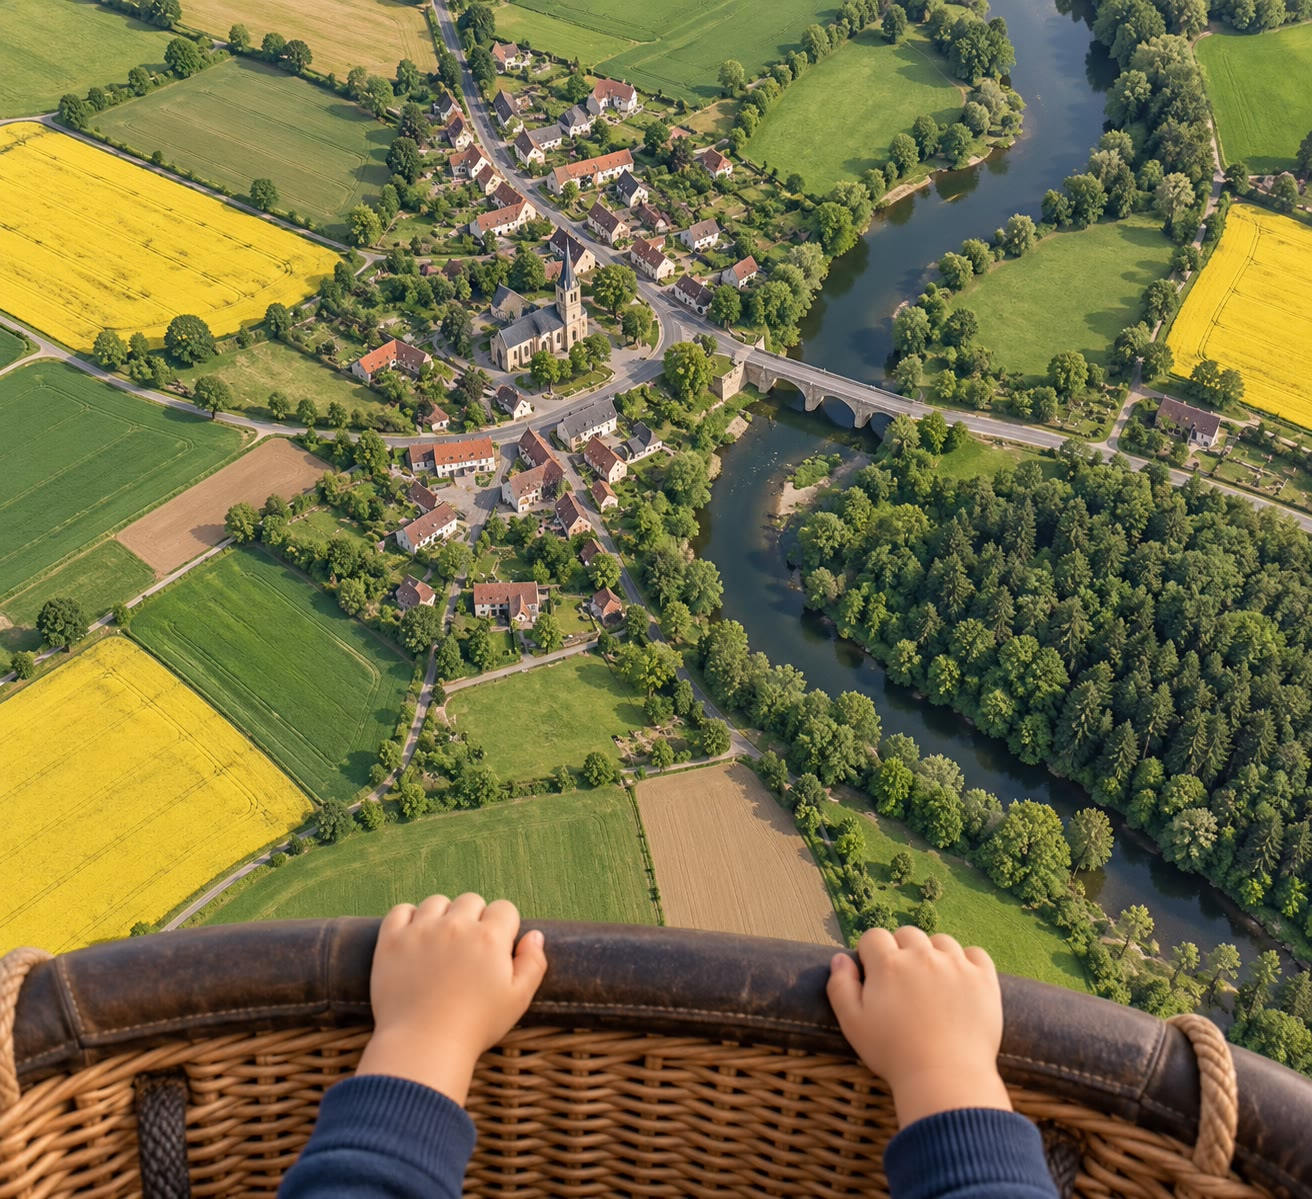
\includegraphics[width=0.62\linewidth]{images/book1/ai/g2-balloon-view.jpg}

{\small El campo visto desde un globo aerostático: campos, un pueblo, una
carretera, un \omterm{def:g1:landscapes-around-us:water}{río} y su puente, todo visto desde arriba.}
\end{omfigure}

\section{Visto de lado, visto desde arriba}

Pon unos bloques de construcción sobre una mesa. Míralos de lado: ves su
altura, y los de atrás quedan escondidos detrás de los de delante. Ahora
ponte de pie y míralos desde arriba: ya no ves lo altos que son, pero ves
exactamente dónde está cada uno y lo separados que están.

\begin{omfigure}
\begin{tikzpicture}[x=1cm, y=1cm, font=\small]
  % side view
  \begin{scope}
    \draw[black!50] (-0.2,0) -- (4.6,0);
    \fill[red!55, draw=black!60] (0.2,0) rectangle (1.2,1.6);
    \fill[ocBlue!55, draw=black!60] (1.6,0) rectangle (3.0,0.8);
    \fill[yellow!70, draw=black!60] (3.4,0) -- (3.9,1.1) -- (4.4,0) -- cycle;
    \node at (2.2,-0.5) {visto de lado};
  \end{scope}
  % from above
  \begin{scope}[shift={(6.4,0)}]
    \draw[black!30, fill=black!3] (-0.2,-0.1) rectangle (4.6,2.3);
    \fill[red!55, draw=black!60] (0.2,0.4) rectangle (1.2,1.4);
    \fill[ocBlue!55, draw=black!60] (1.6,1.0) rectangle (3.0,2.0);
    \fill[yellow!70, draw=black!60] (3.9,0.75) circle (0.5);
    \node at (2.2,-0.5) {visto desde arriba};
  \end{scope}
\end{tikzpicture}

{\small Tres bloques sobre una mesa: un bloque rojo alto, un bloque azul
plano y un cono amarillo. Desde arriba, el cono es un círculo y el bloque
alto es un cuadrado.}
\label{fig:g2:drawing-to-map:blocks}
\end{omfigure}

\begin{definition}[Plano]\label{def:g2:drawing-to-map:plan}
Un \emph{plano}\index{plano} es un dibujo de un lugar pequeño --- una
habitación, una casa, un colegio, un jardín --- tal como se ve desde justo
encima, dibujado más pequeño de lo que es en realidad pero con cada parte en
su sitio.
\end{definition}

\section{Dibujar más pequeño: la escala}

Un aula es demasiado grande para dibujarla tal cual en una hoja de papel. La
dibujamos más pequeña --- pero cada parte debe hacerse más pequeña de la
misma manera, o el \omterm{def:g2:drawing-to-map:plan}{plano} mentirá. Lo más fácil es usar papel
cuadriculado: un cuadrado del papel representa un metro del aula.

\begin{definition}[Escala]\label{def:g2:drawing-to-map:scale}
La \emph{escala}\index{escala} de un \omterm{def:g2:drawing-to-map:plan}{plano} o de un \omterm{def:g2:drawing-to-map:map}{mapa} dice cuánto más
pequeño es el dibujo que el lugar real: qué distancia sobre el terreno
representa una longitud del dibujo. Por ejemplo: \emph{1 cuadrado representa
1 metro}.
\end{definition}

\begin{omfigure}
\begin{tikzpicture}[x=0.75cm, y=0.75cm, font=\scriptsize]
  \draw[black!15] (0,0) grid (10,8);
  \draw[black, line width=1.6pt] (0,0) rectangle (10,8);
  % board on the north wall
  \fill[black!70] (3,7.8) rectangle (7,8);
  % teacher's desk
  \fill[brown!50, draw=black!70] (4,6) rectangle (6,7);
  % pupils' desks: 3 rows of 3
  \foreach \x in {1,4,7} \foreach \y in {1,2.5,4}
    \fill[orange!45, draw=black!70] (\x,\y) rectangle ++(2,1);
  % cupboard
  \fill[ocBlue!40, draw=black!70] (9,5) rectangle (10,8);
  % door (gap) on the east wall, windows on the west wall
  \fill[white] (9.85,1) rectangle (10.15,2);
  \draw[black!70] (10,2) arc[start angle=90, end angle=180, radius=1];
  \foreach \y in {1.5,4.5}
    \draw[ocBlue, line width=2.5pt] (0,\y) -- (0,\y+2);
  % legend
  \begin{scope}[shift={(11,7.2)}]
    \node[anchor=west, font=\small\bfseries] at (0,0.4) {El aula};
    \fill[black!70] (0,-0.25) rectangle (0.8,-0.05); \node[anchor=west] at (1,-0.15) {pizarra};
    \fill[brown!50, draw=black!70] (0,-1.1) rectangle (0.8,-0.7); \node[anchor=west] at (1,-0.9) {mesa del maestro};
    \fill[orange!45, draw=black!70] (0,-1.85) rectangle (0.8,-1.45); \node[anchor=west] at (1,-1.65) {mesa de alumno};
    \fill[ocBlue!40, draw=black!70] (0,-2.6) rectangle (0.8,-2.2); \node[anchor=west] at (1,-2.4) {armario};
    \draw[ocBlue, line width=2.5pt] (0,-3.15) -- (0.8,-3.15); \node[anchor=west] at (1,-3.15) {ventana};
    \draw[black!70] (0.8,-3.95) arc[start angle=0, end angle=90, radius=0.6]; \draw[black, line width=1.6pt] (0.2,-3.95) -- (0.8,-3.95); \node[anchor=west] at (1,-3.7) {puerta};
    \draw[black!15] (0,-4.9) rectangle (0.75,-4.15);
    \node[anchor=west] at (1,-4.53) {1 cuadrado = 1 metro};
    \pic[scale=0.7, transform shape] at (0.7,-6.2) {compassrose};
  \end{scope}
\end{tikzpicture}

{\small El \omterm{def:g2:drawing-to-map:plan}{plano} de un aula en papel cuadriculado, con su título, su
\omterm{def:g2:drawing-to-map:legend}{leyenda}, su \omterm{def:g2:drawing-to-map:scale}{escala} y su \omterm{def:g2:drawing-to-map:directions}{rosa de los vientos}. La pared norte, la de la
pizarra, está arriba.}
\label{fig:g2:drawing-to-map:classroom}
\end{omfigure}
% (exercise data: an invented classroom of 10 m by 8 m)

\begin{method}[Medir en un plano]\label{met:g2:drawing-to-map:measure}
Para hallar una longitud real en un plano dibujado sobre cuadrados:
\begin{enumerate}
  \item cuenta los cuadrados a lo largo de la longitud que quieres;
  \item lee la \omterm{def:g2:drawing-to-map:scale}{escala}: cuánto representa un cuadrado;
  \item da la respuesta en metros (o en kilómetros en un \omterm{def:g2:drawing-to-map:map}{mapa}).
\end{enumerate}
\end{method}

\begin{example}[¿Cuánto mide de largo el aula?]\label{ex:g2:drawing-to-map:length}
A lo largo de la pared norte del \omterm{def:g2:drawing-to-map:plan}{plano} hay 10 cuadrados. Un cuadrado
representa 1 metro, así que el aula mide 10 metros de largo. A lo largo de
la pared oeste hay 8 cuadrados: mide 8 metros de ancho. La pizarra ocupa 4
cuadrados de la pared norte: mide 4 metros de largo.
\end{example}

\begin{omfigure}
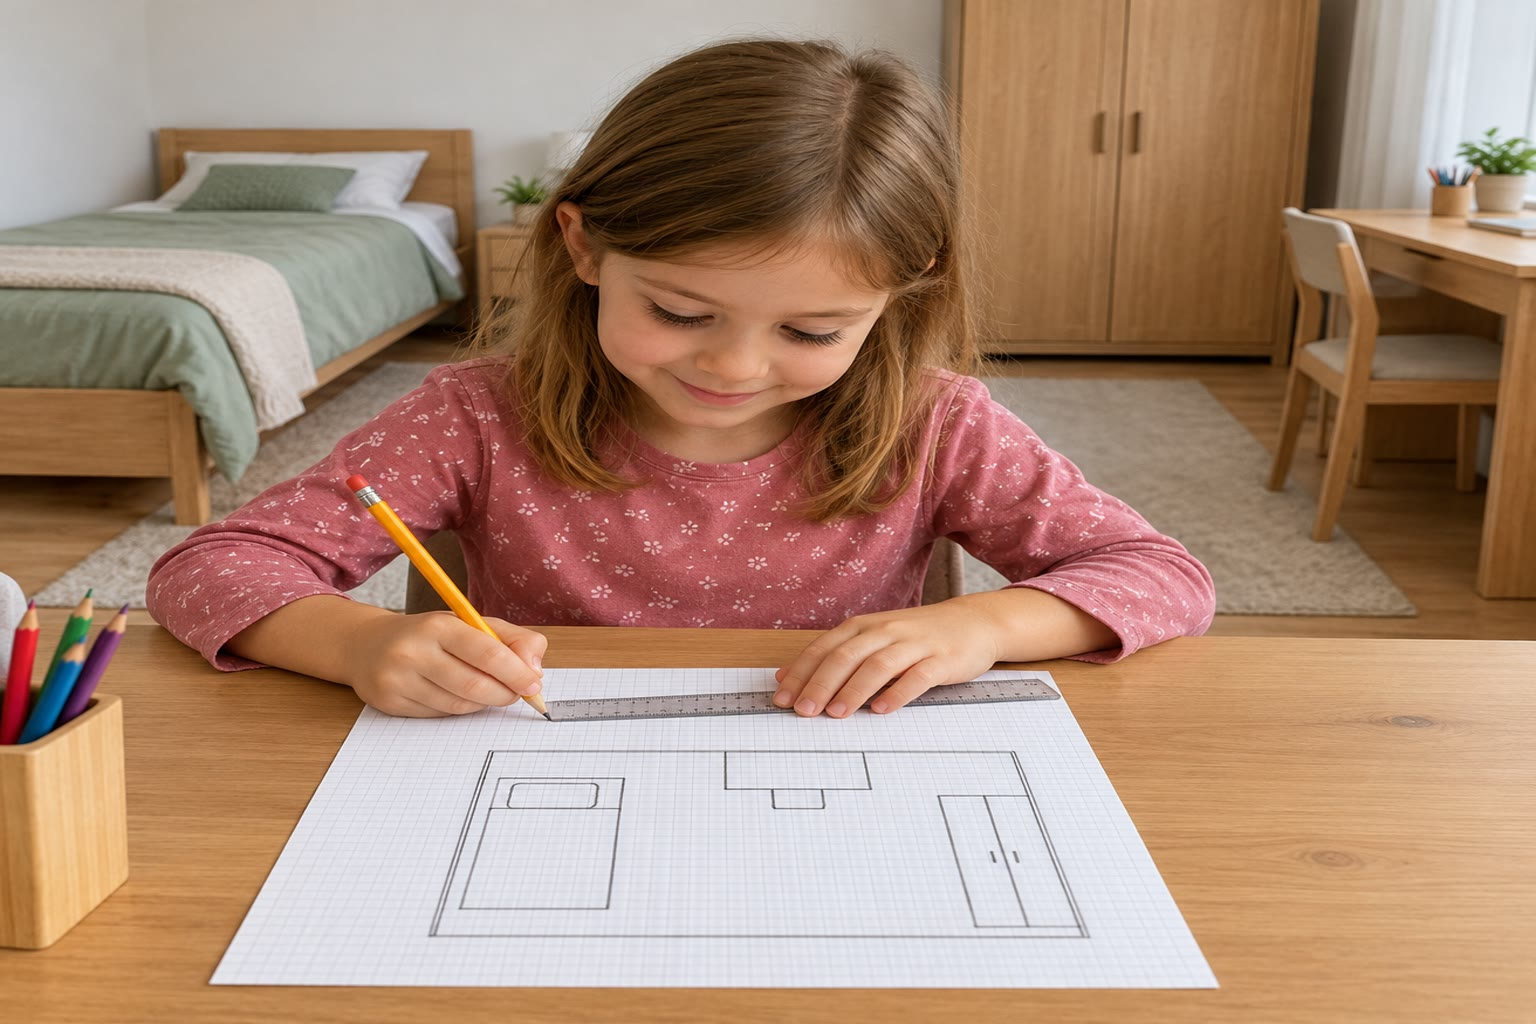
\includegraphics[width=0.55\linewidth]{images/book1/ai/g2-bedroom-plan.jpg}

{\small Dibujamos el \omterm{def:g2:drawing-to-map:plan}{plano} de un dormitorio en papel cuadriculado.}
\end{omfigure}

\section{Del plano al mapa}

Un \omterm{def:g2:drawing-to-map:plan}{plano} muestra un lugar pequeño. Cuando dibujamos un lugar más grande
--- una ciudad entera, un \omterm{def:g1:landscapes-around-us:landform}{valle}, un país ---, dibujamos un \omterm{def:g2:drawing-to-map:map}{mapa}.

\begin{definition}[Mapa]\label{def:g2:drawing-to-map:map}
Un \emph{mapa}\index{mapa} es un dibujo de una gran parte de la superficie
de la Tierra, vista desde arriba y dibujada mucho más pequeña de lo que es
en realidad.
\end{definition}

En un \omterm{def:g2:drawing-to-map:map}{mapa}, una casa es demasiado pequeña para dibujarla tal como es, así
que quienes hacen los \omterm{def:g2:drawing-to-map:map}{mapas} usan pequeños signos: un punto para una granja,
una línea azul para un \omterm{def:g1:landscapes-around-us:water}{río}, una mancha verde para un bosque. El significado
de cada signo se da en un recuadro junto al \omterm{def:g2:drawing-to-map:map}{mapa}.

\begin{definition}[Leyenda]\label{def:g2:drawing-to-map:legend}
Un \emph{signo convencional}\index{signo convencional} es un pequeño signo
que representa una clase de cosa en un plano o en un \omterm{def:g2:drawing-to-map:map}{mapa}. La
\emph{leyenda}\index{leyenda} es el recuadro que muestra cada signo del \omterm{def:g2:drawing-to-map:map}{mapa}
con su significado.
\end{definition}

\section{Orientarse: los cuatro puntos cardinales y la rosa de los vientos}

Para decir dónde está algo, ``a la izquierda'' o ``a la derecha'' no basta:
lo que está a tu izquierda está a la derecha de alguien que te mira de
frente. La gente usa cuatro direcciones que son las mismas para todos:
norte, este, sur y oeste. Ya las has visto en los libros de física, con la
brújula. Por la mañana el Sol sale por el este y por la tarde se pone por el
oeste; el norte y el sur están a medio camino entre los dos, uno frente al
otro.

\begin{omfigure}
\begin{tikzpicture}[font=\small]
  \pic[scale=1.5, transform shape] at (0,0) {compassrose};
  \node[align=left, anchor=west, font=\small] at (2.6,0.3)
    {N = norte (arriba en casi todos los mapas)\\E = este (a la derecha)\\S = sur (abajo)\\O = oeste (a la izquierda)};
\end{tikzpicture}

{\small Una \omterm{def:g2:drawing-to-map:directions}{rosa de los vientos}. Entre el norte y el este está el noreste;
entre el sur y el oeste, el suroeste.}
\label{fig:g2:drawing-to-map:rose}
\end{omfigure}

\begin{definition}[Rosa de los vientos]\label{def:g2:drawing-to-map:directions}
Una \emph{rosa de los vientos}\index{rosa de los vientos} es la estrella
dibujada en un \omterm{def:g2:drawing-to-map:map}{mapa} que muestra las direcciones norte, este, sur y oeste. En
casi todos los \omterm{def:g2:drawing-to-map:map}{mapas} el norte está arriba, el este a la derecha, el sur
abajo y el oeste a la izquierda.
\end{definition}

\begin{safety}
No mires nunca al Sol para encontrar el este o el oeste: puede dañarte los
ojos para siempre. Mira las sombras, o usa una brújula.
\end{safety}

\section{Leer un mapa de verdad}

Todo buen \omterm{def:g2:drawing-to-map:map}{mapa} tiene cuatro partes: un \textbf{título} que dice lo que
muestra el \omterm{def:g2:drawing-to-map:map}{mapa}, una \textbf{\omterm{def:g2:drawing-to-map:legend}{leyenda}}, una \textbf{\omterm{def:g2:drawing-to-map:scale}{escala}} y una
\textbf{\omterm{def:g2:drawing-to-map:directions}{rosa de los vientos}} (o al menos una flecha que señala el norte).
Aquí tienes el \omterm{def:g2:drawing-to-map:map}{mapa} de un \omterm{def:g1:landscapes-around-us:landform}{valle} entre \omterm{def:g1:landscapes-around-us:landform}{colinas}, las Colinas de Varden. Es el
\omterm{def:g1:landscapes-around-us:landform}{valle} inventado que encontrarás una y otra vez en este libro y en los
siguientes, cada vez dibujado con más detalle.

\begin{omfigure}
\begin{tikzpicture}
\begin{axis}[width=9.6cm, scale only axis,
    xmin=0, xmax=10, ymin=0, ymax=8, axis equal image,
    xtick={0,...,10}, ytick={0,...,8}, xticklabels={}, yticklabels={},
    grid=major, grid style={black!20}, major tick length=0pt,
    axis background/.style={fill=green!12!omLithAlluv},
    title={\textbf{Las Colinas de Varden}}]
  \addplot[fill=omHypsLandD, draw=omHypsLandE!80!black, line width=0.4pt, fill opacity=0.85,
    unbounded coords=jump, even odd rule] table {figdata/out/grade-2-varden_plan-hills.dat};
  \addplot[fill=green!45!black!55, draw=green!35!black, line width=0.4pt] table {figdata/out/grade-2-varden_plan-wood.dat};
  \addplot[ocBlue!85!black, line width=2.2pt] table {figdata/out/shared-region-river.dat};
  \addplot[red!65!black, line width=1.3pt] table {figdata/out/grade-2-varden_plan-road.dat};
  \fill[black] (axis cs:5.012,3.414) ++(-3pt,-4pt) rectangle ++(6pt,8pt);
  \fill[white] (axis cs:5.012,3.414) ++(-1.6pt,-4pt) rectangle ++(3.2pt,8pt);
  \fill[brown!70!black] (axis cs:2.5,3.5) ++(-3.5pt,-3.5pt) rectangle ++(7pt,7pt);
  \fill[red!70!black] (axis cs:7.5,5.5) ++(-5pt,-3pt) rectangle ++(4pt,4pt);
  \fill[red!70!black] (axis cs:7.5,5.5) ++(1pt,-3pt) rectangle ++(4pt,4pt);
  \fill[red!70!black] (axis cs:7.5,5.5) ++(-2pt,2pt) rectangle ++(4pt,4pt);
\end{axis}
\begin{scope}[shift={(10.2,6.4)}, font=\small]
  \node[anchor=west, font=\small\bfseries] at (-0.1,0.55) {Leyenda};
  \fill[omHypsLandD, draw=omHypsLandE!80!black] (0,-0.2) rectangle (0.7,0.15); \node[anchor=west] at (0.85,0) {colinas};
  \fill[green!45!black!55] (0,-0.85) rectangle (0.7,-0.5); \node[anchor=west] at (0.85,-0.67) {bosque};
  \draw[ocBlue!85!black, line width=2.2pt] (0,-1.35) -- (0.7,-1.35); \node[anchor=west] at (0.85,-1.35) {río};
  \draw[red!65!black, line width=1.3pt] (0,-2.0) -- (0.7,-2.0); \node[anchor=west] at (0.85,-2.0) {carretera};
  \fill[black] (0.25,-2.8) rectangle (0.45,-2.5); \fill[white] (0.3,-2.8) rectangle (0.4,-2.5); \node[anchor=west] at (0.85,-2.65) {puente};
  \fill[brown!70!black] (0.23,-3.45) rectangle (0.47,-3.21); \node[anchor=west] at (0.85,-3.33) {granja};
  \foreach \dx/\dy in {0.12/-4.1, 0.33/-4.1, 0.22/-3.92}
    \fill[red!70!black] (\dx,\dy) rectangle ++(0.13,0.13);
  \node[anchor=west] at (0.85,-3.98) {pueblo};
  \draw[black!40] (0,-4.95) rectangle (0.5,-4.45); \node[anchor=west, align=left] at (0.85,-4.7) {1 cuadrado\\= 1 kilómetro};
  \pic[scale=0.75, transform shape] at (0.8,-6.5) {compassrose};
\end{scope}
\end{tikzpicture}

{\small Un \omterm{def:g2:drawing-to-map:map}{mapa} sencillo de las Colinas de Varden, con su título, su
\omterm{def:g2:drawing-to-map:legend}{leyenda}, su \omterm{def:g2:drawing-to-map:scale}{escala} y su \omterm{def:g2:drawing-to-map:directions}{rosa de los vientos}. El \omterm{def:g1:landscapes-around-us:water}{río} corre de oeste a este.}
\label{fig:g2:drawing-to-map:varden}
\end{omfigure}
% (figdata/grade-2/varden_plan.py; the region: figdata/shared/region.py)

\begin{method}[Leer un mapa]\label{met:g2:drawing-to-map:read}
\begin{enumerate}
  \item Lee el título: ¿qué lugar muestra el \omterm{def:g2:drawing-to-map:map}{mapa}?
  \item Lee la \omterm{def:g2:drawing-to-map:legend}{leyenda}: ¿qué significa cada signo?
  \item Busca la \omterm{def:g2:drawing-to-map:directions}{rosa de los vientos}: ¿dónde está el norte?
  \item Lee la \omterm{def:g2:drawing-to-map:scale}{escala} y cuenta cuadrados para hallar distancias.
\end{enumerate}
\end{method}

\begin{example}[De la granja al pueblo]\label{ex:g2:drawing-to-map:farm}
En el \omterm{def:g2:drawing-to-map:map}{mapa} de las Colinas de Varden, la granja está al sur del \omterm{def:g1:landscapes-around-us:water}{río}. Para ir
al pueblo, el granjero toma la carretera hacia el este, cruza el \omterm{def:g1:landscapes-around-us:water}{río} por el
puente y sigue hacia el noreste. El pueblo está 5 cuadrados al este de la
granja y 2 cuadrados al norte: es decir, 5 kilómetros hacia el este y
2 kilómetros hacia el norte.
\end{example}

\section{Ejercicios}

\begin{exercise}[$\star$]\label{exo:g2:drawing-to-map:1}
¿Un \omterm{def:g2:drawing-to-map:plan}{plano} se dibuja tal como se ve de lado o tal como se ve desde arriba?
\end{exercise}

\begin{exercise}[$\star$]\label{exo:g2:drawing-to-map:2}
En el \omterm{def:g2:drawing-to-map:plan}{plano} del aula, ¿qué está dibujado en azul en la pared oeste? ¿Qué hay
en la esquina noreste?
\end{exercise}

\begin{exercise}[$\star$]\label{exo:g2:drawing-to-map:3}
Nombra las cuatro partes que debería tener todo buen \omterm{def:g2:drawing-to-map:map}{mapa}.
\end{exercise}

\begin{exercise}[$\star$]\label{exo:g2:drawing-to-map:4}
En casi todos los \omterm{def:g2:drawing-to-map:map}{mapas}, ¿qué dirección está arriba? ¿Cuál está a la
izquierda?
\end{exercise}

\begin{exercise}[$\star$]\label{exo:g2:drawing-to-map:5}
En el \omterm{def:g2:drawing-to-map:plan}{plano} del aula, una mesa de alumno ocupa 2 cuadrados por 1 cuadrado.
¿Cuánto mide de largo y de ancho una mesa en el aula real?
\end{exercise}

\begin{exercise}[$\star$]\label{exo:g2:drawing-to-map:6}
En el \omterm{def:g2:drawing-to-map:map}{mapa} de las Colinas de Varden, ¿qué representa el cuadrado marrón? ¿Y
la mancha verde?
\end{exercise}

\begin{exercise}[$\star\star$]\label{exo:g2:drawing-to-map:7}
En el \omterm{def:g2:drawing-to-map:map}{mapa} de las Colinas de Varden, ¿el bosque está al norte o al sur del
\omterm{def:g1:landscapes-around-us:water}{río}? ¿Está al este o al oeste de la granja?
\end{exercise}

\begin{exercise}[$\star\star$]\label{exo:g2:drawing-to-map:8}
En el \omterm{def:g2:drawing-to-map:map}{mapa} de las Colinas de Varden, el \omterm{def:g2:drawing-to-map:map}{mapa} entero mide 10 cuadrados de
oeste a este y 8 cuadrados de sur a norte. ¿Cuántos kilómetros son en cada
dirección?
\end{exercise}

\begin{exercise}[$\star\star$]\label{exo:g2:drawing-to-map:9}
En el \omterm{def:g2:drawing-to-map:plan}{plano} del aula, ¿cuántas mesas de alumno hay? Un alumno se sienta en
la mesa más cercana a la puerta. ¿Está en el norte o en el sur del aula?
\end{exercise}

\begin{exercise}[$\star\star$]\label{exo:g2:drawing-to-map:10}
Lucas dibuja un \omterm{def:g2:drawing-to-map:plan}{plano} de su dormitorio. Su cama mide 2 metros de largo. Con
la \omterm{def:g2:drawing-to-map:scale}{escala} ``1 cuadrado representa 1 metro'', ¿cuántos cuadrados mide la cama
en su \omterm{def:g2:drawing-to-map:plan}{plano}? Su dormitorio mide 4 metros de largo y 3 metros de ancho:
¿cuántos cuadrados ocupa toda la habitación?
\end{exercise}

\begin{exercise}[$\star\star$]\label{exo:g2:drawing-to-map:11}
Lena dice: ``El \omterm{def:g1:landscapes-around-us:water}{río} está a mi izquierda''. ¿Por qué esto no nos dice dónde
está el \omterm{def:g1:landscapes-around-us:water}{río}? Dilo de otra manera que sea verdad para todos, si Lena está en
la granja de las Colinas de Varden.
\end{exercise}
